\documentclass[11pt,a4paper]{article}
\usepackage[margin=2.3cm]{geometry}
\usepackage[T1]{fontenc}
\usepackage{textcomp}
\input{glyphtounicode}
\pdfgentounicode=1
\usepackage{lmodern}
\usepackage{xcolor}
\usepackage{listings}
\usepackage{tcolorbox}
\usepackage{tikz}
\usepackage{hyperref}
\hypersetup{colorlinks=true, linkcolor=blue!50!black, citecolor=green!40!black}

\definecolor{codebg}{RGB}{248,248,245}
\lstset{
  language=C, basicstyle=\ttfamily\footnotesize, backgroundcolor=\color{codebg},
  keywordstyle=\color{blue!60!black}\bfseries, commentstyle=\color{green!45!black}\itshape,
  stringstyle=\color{red!60!black}, numbers=none, upquote=true,
  frame=single, rulecolor=\color{gray!40}, breaklines=true, columns=fullflexible,
  keepspaces=true, showstringspaces=false
}
\lstdefinestyle{sh}{language=bash, numbers=none, backgroundcolor=\color{black!5}}

\newtcolorbox{keyidea}{colback=blue!4, colframe=blue!45!black, title=Key ideas, fonttitle=\bfseries\small}
\newtcolorbox{experiment}{colback=orange!5, colframe=orange!70!black, title=Experiment, fonttitle=\bfseries\small}

\title{\textbf{OpenMP --- Lesson 1}\\[4pt]\large The parallel region and the fork--join model}
\author{Study notes for Flor Vargas}
\date{November 2026}

\begin{document}
\maketitle

\noindent\textit{\small Sources: Chapman, Jost \& van der Pas~\cite{chapman}, Ch.~2
``Overview of OpenMP'' (fork--join execution model) and Ch.~3 ``Writing a First OpenMP
Program''; the \texttt{parallel} construct in detail is in Ch.~4 ``OpenMP Language Features''.}

\section{The idea}
An OpenMP program starts as an ordinary serial C program with \textbf{one} thread, the
\emph{master} (id~0). When it reaches a \texttt{parallel} directive it \textbf{forks}: a
\emph{team} of threads is created and \emph{every} thread executes the same block of code.
At the end of the block there is an \textbf{implicit barrier}: all threads wait until the
whole team has finished, then the team \textbf{joins} back into the master, and the program
continues serially.

\begin{center}
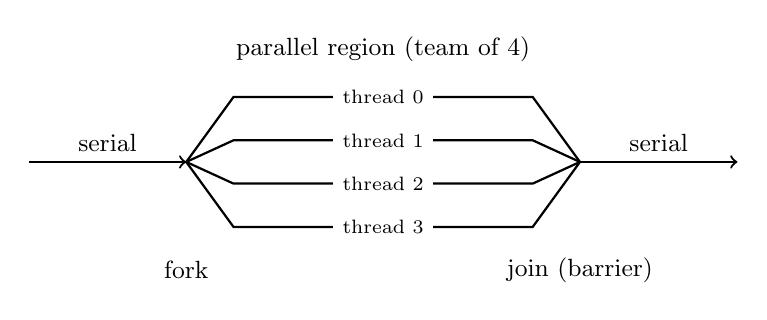
\begin{tikzpicture}[x=1cm,y=0.55cm, thick]
  \draw[->] (0,0) -- (2,0) node[midway,above]{\small serial};
  \foreach \y in {1.5,0.5,-0.5,-1.5} {
    \draw (2,0) -- (2.6,\y) -- (6.4,\y) -- (7,0);
  }
  \node at (4.5,2.6) {\small parallel region (team of 4)};
  \node at (2,-2.5) {\small fork};
  \node at (7,-2.5) {\small join (barrier)};
  \draw[->] (7,0) -- (9,0) node[midway,above]{\small serial};
  \node[font=\scriptsize,fill=white] at (4.5,1.5) {thread 0};
  \node[font=\scriptsize,fill=white] at (4.5,0.5) {thread 1};
  \node[font=\scriptsize,fill=white] at (4.5,-0.5) {thread 2};
  \node[font=\scriptsize,fill=white] at (4.5,-1.5) {thread 3};
\end{tikzpicture}
\end{center}

\section{The three ingredients}
\begin{enumerate}
  \item \textbf{The directive} \texttt{\#pragma omp parallel} placed before a block
        \texttt{\{ \ldots \}}. This is the only construct that creates threads.
  \item \textbf{The runtime library} \texttt{omp.h}:
        \texttt{omp\_get\_thread\_num()} returns the calling thread's id
        ($0,\dots,n-1$); \texttt{omp\_get\_num\_threads()} returns the team size $n$.
  \item \textbf{The compiler flag} \texttt{-fopenmp}. Without it, \texttt{gcc} ignores the
        pragma.
\end{enumerate}
The team size is chosen at run time, most simply with the environment variable
\texttt{OMP\_NUM\_THREADS}. If it is not set, the default is usually the number of cores.

\section{The code}
\lstinputlisting[title=\texttt{hello\_parallel.c}]{hello_parallel.c}

\begin{lstlisting}[style=sh]
gcc -Wall -fopenmp -o hello_parallel hello_parallel.c
OMP_NUM_THREADS=4 ./hello_parallel
\end{lstlisting}
Typical output (your order will differ):
\begin{lstlisting}[style=sh]
before: 1 thread(s) running
  hello from thread 1 of 4
  hello from thread 3 of 4
  hello from thread 2 of 4
  hello from thread 0 of 4
after:  1 thread(s) running
\end{lstlisting}

\begin{keyidea}
\begin{itemize}
  \item Code \emph{outside} the region runs once; code \emph{inside} runs once \emph{per thread}.
  \item The threads run concurrently, so the order of their output is \textbf{not
        deterministic}. Never assume thread 0 goes first.
  \item The barrier at the end of the region guarantees that ``after'' is printed only
        when every thread is done.
  \item Variables declared \emph{inside} the region are private to each thread.
        That is why every thread prints its own \texttt{id}. (Data sharing is Lesson~2.)
\end{itemize}
\end{keyidea}

\section{The experiment}
\begin{experiment}
\textbf{Question:} how does the team size control the work, and is the execution order
reproducible?
\begin{enumerate}
  \item Check how many cores your machine has: \texttt{nproc}.
  \item Run the program with several team sizes:
\begin{lstlisting}[style=sh]
for t in 1 2 4 8; do echo "== $t threads"; OMP_NUM_THREADS=$t ./hello_parallel; done
\end{lstlisting}
  \item Repeat the 4-thread run five times:
\begin{lstlisting}[style=sh]
for r in 1 2 3 4 5; do OMP_NUM_THREADS=4 ./hello_parallel; echo; done
\end{lstlisting}
\end{enumerate}
\textbf{What to observe and answer.}
\begin{enumerate}
  \item The number of ``hello'' lines equals \texttt{OMP\_NUM\_THREADS}, even when it is
        larger than \texttt{nproc}. What does that tell you about threads vs.\ cores?
  \item ``before'' and ``after'' always print once and report 1 thread. Why?
  \item Does the order of the hello lines change between the five repeated runs?
        Why can't OpenMP promise an order?
\end{enumerate}
\end{experiment}

\paragraph{Answers (read after trying).}
(1)~Threads are a software concept; the operating system time-shares them on the
available cores. Asking for more threads than cores is allowed but usually gives no
speed-up.
(2)~Those lines are outside the parallel region, where only the master exists.
(3)~The order usually changes. Each thread is scheduled independently by the OS, so the
interleaving of their \texttt{printf} calls depends on timing. Any program whose
\emph{result} depends on that timing has a \emph{race condition}, the central danger of
shared-memory programming.

\paragraph{Next lesson.} Shared vs.\ private variables: what happens when the threads
write to the \emph{same} variable (\texttt{shared}, \texttt{private} clauses; Chapman
et al., Ch.~4).

\begin{thebibliography}{9}
\bibitem{chapman} B.~Chapman, G.~Jost, and R.~van der Pas. \emph{Using OpenMP: Portable
  Shared Memory Parallel Programming}. MIT Press, Cambridge, MA, 2007.
\end{thebibliography}
\end{document}
